\documentclass[spanish,12pt,letterpaper]{article}

\usepackage[english]{babel}
\usepackage[table]{xcolor}
\usepackage[utf8]{inputenc}
\usepackage{amsmath}
\usepackage{amssymb}
\usepackage{authblk}
\usepackage{csquotes}
\usepackage{enumerate}
\usepackage{float}
\usepackage{forest}
\usepackage{geometry}
\usepackage{graphicx}
\usepackage{listings}
\usepackage{xcolor}

\geometry{
  a4paper,
  total={170mm,257mm},
  left=20mm,
  top=20mm,
}

\definecolor{codegreen}{rgb}{0,0.6,0}
\definecolor{codegray}{rgb}{0.5,0.5,0.5}
\definecolor{codepurple}{rgb}{0.58,0,0.82}
\definecolor{backcolour}{rgb}{0.95,0.95,0.92}

\lstdefinestyle{mystyle}{
  backgroundcolor=\color{backcolour},
  commentstyle=\color{codegreen},
  keywordstyle=\color{orange},
  numberstyle=\tiny\color{codegray},
  stringstyle=\color{codepurple},
  basicstyle=\ttfamily\footnotesize,
  breakatwhitespace=false,
  breaklines=true,
  captionpos=b,
  keepspaces=true,
  numbers=right,
  numbersep=5pt,
  showspaces=false,
  showstringspaces=false,
  showtabs=false,
  tabsize=2
}

\lstset{style=mystyle}

\title{Examen Redes de Computadoras}
\author{Ángel Iván Gladín García\\
  Emiliano Galeana Araujo}
\affil{Facultad de ciencias, UNAM}
\date{Fecha de entrega: Lunes 30 de marzo de 2020}

\begin{document}

\maketitle

\section{Parte teórica}

\subsection{Memoria fotográfica}
\subsubsection{Edificio}
Se decidió utilizar el edificio Poniente (P) de la facultad de Ciencias de la
UNAM.

\subsubsection{Descripción}
El edificio cuenta con 4 pisos que son: Planta Baja, Primer Piso, Segundo Piso y
el Sótano.

\paragraph{Acometida} Es la parte de la instalación eléctrica que se construye
desde las redes de distribución, hasta las instalaciones del usuario.

\paragraph{Cuartos de telecomunicaciones} Área que es utilizada para el uso
exclusivo de equipo asociado  con el sistema de cableado de telecomunicaciones.

\paragraph{Racks} Racks de cada cuarto (Incluyendo Patch Panels) Estructura que
permite sostener un dispositivo tecnológico. Tenemos en el cuarto de
telecomunicaciones, y en los acces points de cada piso. El diagrama de packet
tracer muestra solo una columna, la configuración del rack, se encuentra abajo.
El diagrama, supone distintos pisos.

\paragraph{Switches} Switches de acceso, distribución y core. Representan el
perímetro de la red, por dónde entra o sale el tráfico de la red en cuestión.

\paragraph{Ruteador} Dispositivo empleado a la hora de la interconexión de una
red de ordenadores.

El siguiente diagrama representa al edificio P, con algunas modificaciones para
poder hacer ejemplos más claros.

Los cuadrados chiquitos que engloban computadoras, represenatan salones, y los
rectángulos horizontales, representan los pisos del edificio.

Para las VLAN, se usararon las configuraciones desde el \texttt{CLI} de los
switches.

\begin{center}
  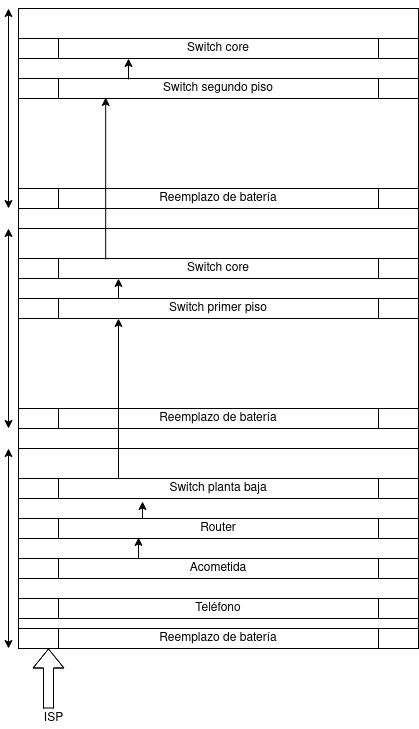
\includegraphics[scale=.6]{rackP.png}
\end{center}


\begin{center}
  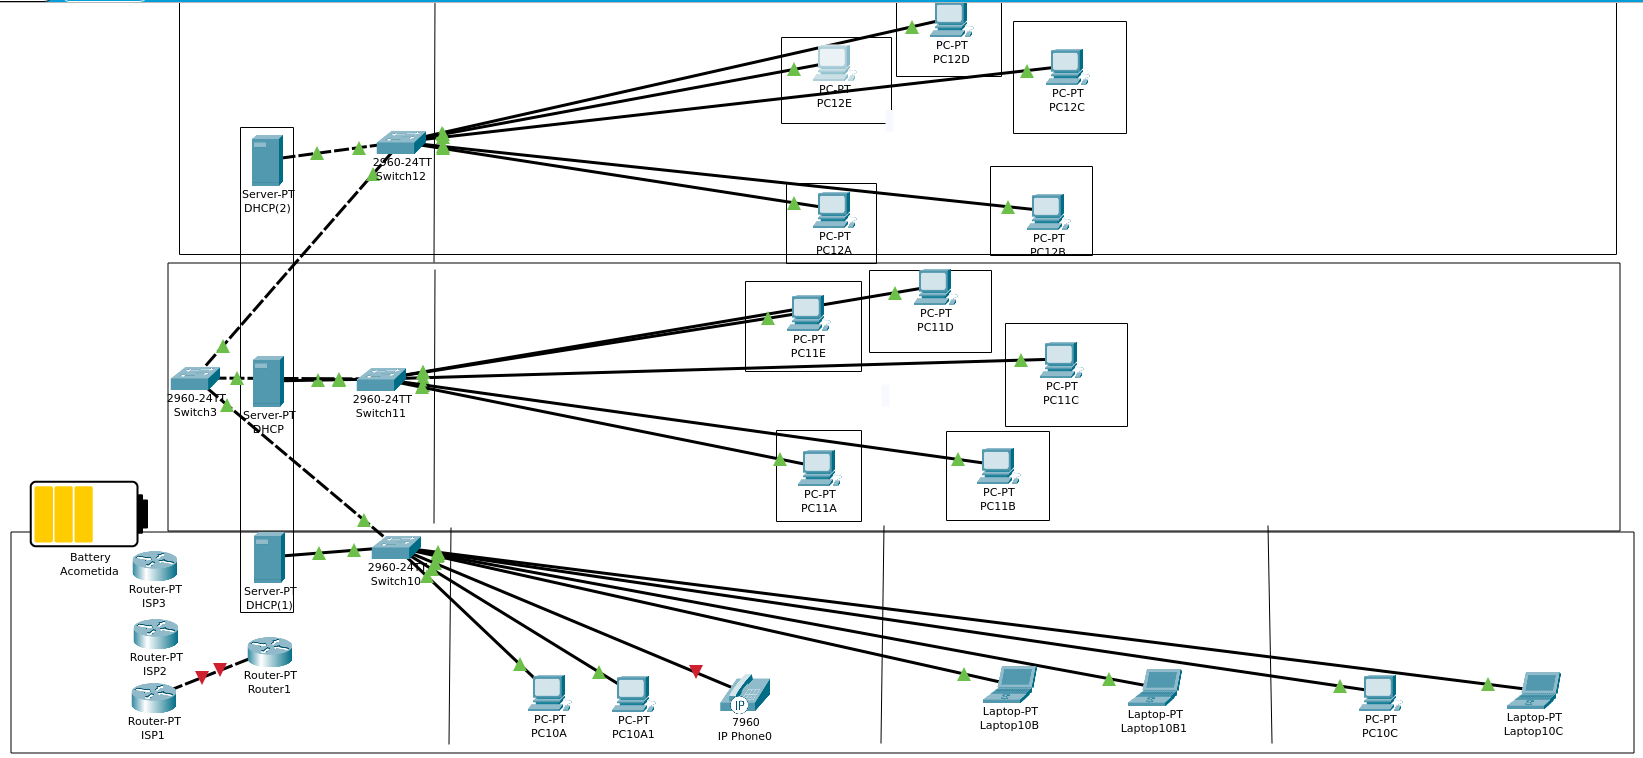
\includegraphics[scale=.28]{nuevoPP.png}
\end{center}

\subsubsection{Inventario}
Debido a que este un ejemplo meramente de demostración, es importante aclarar que
la siguiente tabla no fue hecha con datos reales.

\begin{table}[H]
  \centering
  \begin{tabular}{| c | c | c | c | c |}\hline
    Equipo & IPs & Máscara de red & Gateway & VLAN \\ \hline
    Switch10 & -----  & ----- & ----- & 10 \\ \hline 
    Switch11 & -----  & ----- & ----- & 11 \\ \hline
    Switch12 & -----  & ----- & ----- & 12 \\ \hline
    PC10A  & 10.10.10.13  & 255.0.0.0 & 10.10.10.4 & 10  \\ \hline
    PC10A1 & 10.10.10.17  & 255.0.0.0 & 10.10.10.4 & 10 \\ \hline
    PC10C  & 10.10.10.38  & 255.0.0.0 & 10.10.10.4 & 10 \\ \hline
    PC11A  & 168.10.0.7  & 255.255.0.0 & 168.10.0.4 & 11 \\ \hline
    PC11B  & 168.10.0.8  & 255.255.0.0 & 168.10.0.4 & 11 \\ \hline
    PC11C  & 168.10.0.9 & 255.255.0.0 & 168.10.0.4 & 11 \\ \hline
    PC11D  & 168.10.0.21 & 255.255.0.0 & 168.10.0.4 & 11 \\ \hline
    PC11E  & 168.10.0.18 & 255.255.0.0 & 168.10.0.4 & 11 \\ \hline
    PC12A  & 192.168.10.14 & 255.255.255.0 & 192.168.10.2 & 12 \\ \hline
    PC12B  & 192.168.10.8  & 255.255.255.0 & 192.168.10.2 & 12 \\ \hline
    PC12C  & 192.168.10.9  & 255.255.255.0 & 192.168.10.2 & 12 \\ \hline
    PC12D  & 192.168.10.10 & 255.255.255.0 & 192.168.10.2 & 12 \\ \hline
    PC12E  & 192.168.10.11 & 255.255.255.0 & 192.168.10.2 & 12 \\ \hline
    Laptop10B  & 10.10.10.18 & 255.0.0.0 & 10.10.10.4 & 10 \\ \hline
    Laptop10B1  & 10.10.10.25 & 255.0.0.0 & 10.10.10.4 & 10 \\ \hline
    Laptop10C  & 10.10.10.43 & 255.0.0.0 & 10.10.10.4 & 10 \\ \hline
  \end{tabular}
  \caption{Inventario de direcciones IP.}
\end{table}


\subsubsection{Tabla de rutas}
%% https://www.youtube.com/watch?v=VbRRWTMh1GA quizá ayude


\begin{table}[H]
  \centering
  \begin{tabular}{| c | c | c | c | c |}\hline
    Equipo & IPs & Máscara de red & Gateway & VLAN \\ \hline
    Router0 & 192.0.2.0/24 & ----- & 10 & \\
    & 198.51.100.0/24 & ----- &  & \\
    & 203.0.113.0/24 & ----- &  & \\\hline
  \end{tabular}
  \caption{Tabla de rutas del router.}
\end{table}
\section{Parte práctica}
\subsection{Considerar una red de la siguiente forma}
\begin{center}
  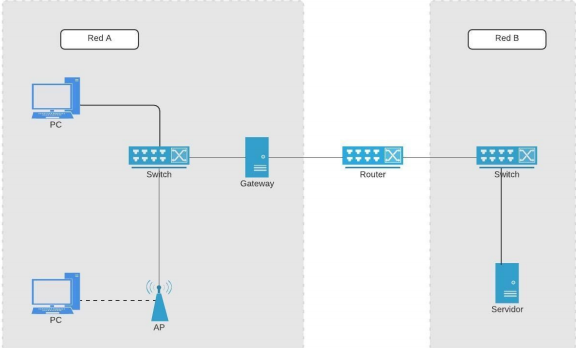
\includegraphics[scale=.75]{red.png}
\end{center}
Llevar a cabo lo siguiente:

  Recordemos lo siguiente:
  \begin{itemize}
  \item Clase A: 0.0.0.0 hasta 127.255.255.255
  \item Clase B: 128.0.0.0 hasta 191.255.255.255
  \item Clase C: 192.0.0.0 hasta 223.255.255.255
  \end{itemize}
  
\begin{itemize}
  
\item Asignar direcciones de un \textit{segmento privado de clase B} a los
  equipos de la Red A.

  \begin{table}[H]
    \centering
    \begin{tabular}{|c | c |}\hline
      Nombre & Asignación     \\ \hline
      PC(up) & 172.16.0.3     \\ \hline
      PC(down) & 172.16.1.2   \\ \hline    
      AP & 172.16.1.1         \\ \hline
      Switch & 172.16.0.2     \\ \hline
    \end{tabular}
  \end{table}

\item Establecer la dirección del \textit{gateway} en la Red A.

  Getaway : 172.16.0.1
  
\item Indica la configuración de red que se debe usar en los equipos de la Red A
  (\textit{dirección de red, gateway, máscara de subred} y otros que consideres
  necesarios).

  \begin{table}[H]
    \centering
    \begin{tabular}{| c | c | c |}\hline
      Dispositivo & Nombre & Asignación\\ \hline
      PC(up) & & \\ \hline
      & Dirección de red & 172.16.0.3 \\ \hline
      & Getaway & 172.16.0.2 \\ \hline
      & Máscara de sub red & 255.255.0.0 \\ \hline
    \end{tabular}
  \end{table}

  \begin{table}[H]
    \centering
    \begin{tabular}{| c | c | c |}\hline
      Dispositivo & Nombre & Asignación\\ \hline
      Switch & & \\ \hline
      & Dirección de red & 172.16.0.2 \\ \hline
      & Getaway & 172.16.0.1 \\ \hline
      & Máscara de sub red & 255.255.0.0 \\ \hline
    \end{tabular}
  \end{table}

  \begin{table}[H]
    \centering
    \begin{tabular}{| c | c | c |}\hline
      Dispositivo & Nombre & Asignación\\ \hline
      AP & & \\ \hline
      & Getaway & 172.16.0.2 \\ \hline
      & Máscara de sub red & 255.255.0.0 \\ \hline
      & IP-WAN & 172.16.1.1 \\ \hline
      & IP-LAN & 172.16.2.2 \\ \hline
    \end{tabular}
  \end{table}

  \begin{table}[H]
    \centering
    \begin{tabular}{| c | c | c |}\hline
      Dispositivo & Nombre & Asignación\\ \hline
      PC(down) & & \\ \hline
      & Dirección de red & 172.16.1.2 \\ \hline
      & Getaway & 172.16.0.2 \\ \hline
      & Máscara de sub red & 255.255.0.0 \\ \hline
    \end{tabular}
  \end{table}

\item Hacer uso de un \textit{segmento de red público de clase C} en los equipos
  de la Red B.

  \begin{table}[H]
    \centering
    \begin{tabular}{|c | c |}\hline
      Nombre & Asignación \\ \hline
      Switch & 192.0.0.2  \\ \hline
      Server & 192.0.0.3   \\ \hline   
    \end{tabular}
  \end{table}
  
\item Establecer la dirección del \textit{gateway} en la Red B.

  Getaway : 192.0.0.1
  
\item Indica la configuración de red que se debe usar en el servidor de la Red B
  (\textit{dirección de red, gateway, máscara de subred} y otros que consideres
  necesarios).
  
  \begin{table}[H]
    \centering
    \begin{tabular}{| c | c | c |}\hline
      Dispositivo & Nombre & Asignación\\ \hline
      Switch & & \\ \hline
      & Dirección de red & 192.0.0.2 \\ \hline
      & Getaway & 192.0.0.1 \\ \hline
      & Máscara de sub red & 255.255.255.0 \\ \hline
    \end{tabular}
  \end{table}

  \begin{table}[H]
    \centering
    \begin{tabular}{| c | c | c |}\hline
      Dispositivo & Nombre & Asignación\\ \hline
      Server & & \\ \hline
      & Dirección de red & 192.0.0.3 \\ \hline
      & Getaway & 192.0.0.1 \\ \hline
      & Máscara de sub red & 255.255.255.0 \\ \hline
    \end{tabular}
  \end{table}
  
\item Asignar una \textit{dirección de red} a las interfaces correspondientes del
  \textit{router}, de acuerdo a las redes conectadas.

  \begin{table}[H]
    \centering
    \begin{tabular}{| c | c |}\hline
      RED & Dirección \\ \hline
      A & 172.16.0.1\\ \hline
      B & 192.0.0.1 \\ \hline
    \end{tabular}
  \end{table}  
  
\item Incluir en el diagrama un \textit{DNS} en una red independiente, haciendo
  uso de un segmento de \textit{red de clase C}, con direcciones públicas.

Haciendo uso del segmento de clase 192.0.0.0/24, tenemos lo siguiente:
  
  \begin{table}[H]
    \centering
    \begin{tabular}{| c | c |}\hline
      Nombre & Dirección \\ \hline
      google.com & 192.0.0.1 \\ \hline
      facebook.com & 192.0.0.2 \\ \hline
      youtube.com & 192.0.0.3 \\ \hline
      twitter.com & 192.0.0.4 \\ \hline
      instagram.com & 192.0.0.5 \\ \hline
    \end{tabular}
  \end{table}

  Por lo que el diagrama se vería de la siguiente manera:

  \begin{center}
  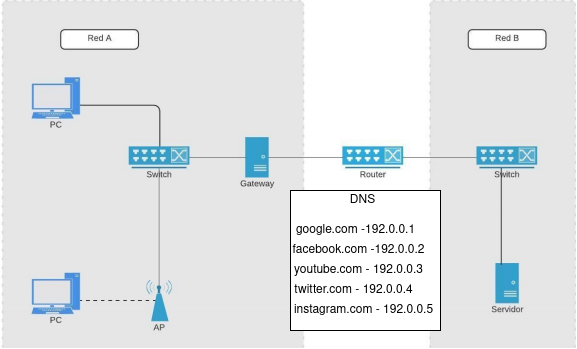
\includegraphics[scale=.75]{DNS.png}
\end{center}  
  
\item Considerando que todos los clientes y servidores involucrados son equipos
  Linux, indica la forma en la que se debe establecer la configuración de
  \textit{red estática} y la configuración necesaria para llevar a cabo la
  \textit{resolución de nombres} en el sistema (archivos y comandos necesarios).

  Existen dos maneras de hacerlo, de forma persistente y por la sesión.

  \begin{itemize}
  \item Persistente:
    \begin{enumerate}
    \item El archivo a utilizar: \texttt{/etc/network/interfaces}
    \item \texttt{auto [interfaz]} configurar que las interfaces se configuren al
      inicio del sistema.
    \item \texttt{iface [interfaz] inet static} para configurarla estáticamente.
    \item Escribimos los siguientes datos con las direcciones necesarias, en caso
      de no tener algún dato, se puede comentar o no poner:
      \begin{itemize}
      \item \texttt{adreess [dirección]}
      \item \texttt{netmask [máscara]}
      \item \texttt{network [red de pertenencia]}
      \item \texttt{broadcast [dirección de broadcast]}
      \item \texttt{gateway [gateway a tomar]}
      \end{itemize}
    \item Podemos aplicar los cambios a todas las interfaces disponibles o, como
      solamente editamos una, hacemos lo siguiente: \texttt{ifdown [intefaz];
        ifup [interfaz]}
    \item \texttt{ifconfig -a} para ver los cambios.
    \end{enumerate}
  \item Sesión:
    \begin{enumerate}
    \item \texttt{ifconfig -a} nos da la información de todas las interfaces de
      red.
    \item Seleccionamos la interfaz que queramos configurar.
    \item \texttt{ifconfig [interfaz] inet 0.0.0.0 down}, quitamos ip y bajamos
      la interfaz (No hacerla disponible para conexiones).
    \item \texttt{ifconfig} muestra todas las interfaces que están arriba.
    \item \texttt{ifconfig [interfaz] inet [dirección] netmask [máscaa] up} con
      esto configuramos otra dirección ip.
    \item \texttt{ifconfig [interfaz]} para verificar lo que hicimos.
    \end{enumerate}
  \end{itemize}
  
\item Por cuestiones de simplicidad, asignar a cada dispositivo  una
  \textit{dirección física de 4 números hexadecimales}.

  \begin{table}[H]
    \centering
    \begin{tabular}{| c | c |}\hline
      Nombre & Dirección \\ \hline
      PC(up) & 53-34-1A-45-59-4C \\ \hline
      PC(down) & 29-D3-C2-4D-1F-21 \\ \hline
      Switch(A) & 2E-DD-8E-4B-F9-B1 \\ \hline
      AP & AD-F8-EF-E9-BD-A4 \\ \hline
      Gateway & 11-C4-6E-C5-83-02 \\ \hline
      Router & 95-73-E3-A7-9B-35 \\ \hline
      Switch(B) & 0F-49-AD-EB-13-06 \\ \hline
      Server & 91-73-35-CA-C9-8C \\ \hline
    \end{tabular}
  \end{table}  
  
\item Explicar con detalle el procedimiento para llevar a cabo la conexión entre
  una computadora de la Red A al servidor de la Red B, considerando lo siguiente:
  \begin{itemize}
  \item Se debe establecer el nombre del servidor con base en tu nombre y
    apellidos.    
    jose-luis.torres.local o juan.camacho.local
  \item El servidor de la Red B cuenta con una aplicación de "servidor Web" el
    cual solamente acepta peticiones mediante \textit{HTTP} version 1.1 en el
    puerto 54321.
  \item El cliente establecerá una conexión para obtener el documento /paginas
    /directorio.html.
  \item El cliente debe hacer uso de un puerto, fuera del rango establecido para
    los "puertos bien conocidos" y "puertos registrados", para llevar a cabo la
    conexión.
  \item El \textit{gateway} de la Red A implementa \textit{NAT}, haciendo uso de
    una dirección de un segmento de \textit{clase C}.
  \item Se debe incicar detalladamente los passos que se siguen en el cliente de
    la Red A que hacen uso de una conexión con un \textit{medio guiado}, para
    establecer la conexión con el servidor, incluyendo los \textit{bloques de
      datos} que se general al pasar por cada una de las capas de TCP/IP. Se debe
    mostrar la forma en la que se aplica el ``encapsulamiento'' (En las clases se
    presentaron ejemplos de esto)
  \item En la \textit{Capa de Enlace} se debe considerar el uso de ``relleno de
    bits'' para llevar a cabo el \textit{envío de tramas}.
  \item Se debe mostrar la forma en la que se ``desencapsulan'' los paquetes al
    llegar al \textit{router} y la forma en la que se vuelven ``encapsular'' para
    su reenvío.
  \end{itemize}

  \begin{enumerate}
  \item angel-gladin-emiliano-galeana.local quiere conectarse al servidor con
    dirección \texttt{192.0.0.3}.
  \item La computadora (PC(down)), pregunta al DNS en el AP si conoce la
    dirección, como no la conoce.
  \item El AP, le pregunta al Switch si conoce la dirección.
  \item El Switch le pregunta al Gateway (Todo esto, porque nadie ha conocido la
    dirección final).
  \item El Gateway le pergunta al Router, y este, le dice que lo puede redirigir
    a donde cree que podría estar la dirección.
  \item Entra al Switch(B) y le pregunta si conoce la dirección, este dice que si
    y se conecta con el Servidor.
  \item Se verifica que el puerto 54321 esté habilitado para aceptar peticiones.
  \item Se regresan señales para indicarle a angel-gladin-emiliano-galeana.local
    que se estableció una conexión.
  \end{enumerate}
\end{itemize}

\subsection{Explicar cuáles son las características que debe tener un código para
  permitir llevar a cabo \textit{detección} o \textit{corrección} de errores}

Recordemos los tipos de errores que podemos tener:
\begin{itemize}
\item De bit: Ocurre cuando únicamente un bit de una unidad de datos cambia. (Por
  ejemplo, cambia de 0 a 1 o viceversa).
\item De ráfaga: Este error ocurre cuando dos o más bits de la unidad de datos
  han cambiado. En estos errores no necesariamente tenemos cambios en bits
  consecutivos.
\end{itemize}

Para detectar estos errores, podemos hacer uso de la \textit{redundancia}, que,
consiste en enviar dos veces cada unidad de datos, así podemos hacer una
comparación bit a bit entre ambos datos y detectar si hay errores. Para aplicar
esta técnica, podemos añadir al flujo de datos un grupo pequeño de bits al final
de cada unidad, a estos los llamamos bits redundantes y los descartams una vez
que se compruebe la integridad de la transmisión.

Para la correción de errores, podemos hacerlo de dos maneras, si existe un error,
podemos pedir al emisor que retransmita la información, la segunda opción es que
el receptor los corrija.

En este contexto, responde las siguientes preguntas:
\begin{itemize}
\item ¿Qué características debe tener un código para permitir la detección de
  errores de un máximo de n bits?

  Como se explicó antes, podríamos mandar la información dos veces y compararla,
  y así, detectar errores. Pero la más usada, como también se mencionó, es el uso
  de los bits de redundancia. Lo que se requiere del código para permitir la
  detección es que tenga $n$ bits más que nos ayuden a verificar si existe un
  error. Esto haría el mensaje más largo, pero más sencillo el detectar si existe
  o no un error.
  
\item ¿Qué características debe tener un código para permitir la corrección de
  errores de un máximo de n bits?

  Para poder llevar a cabo la correción de errores, (Hablando en errores de un
  bit) necesitamos saber cuál fue el bit que se invirtió y usamos los bits de
  redundancia. ¿Cuántos bits de redundancia son necesarios?

  Supongamos que usamos $r$ bits de redundancia, y que $m$ es la cantidad de bits
  de nuestro mensaje, el mensaje a transmitir tiene una longitud de $m+r$ bits. Y
  se necesita que los $r$ bits sean capaces de indicar todas las posibilidades de
  error de 1 bit, incluyendo el no error (Esto son $m+r+1$ posibilidades).
  Sabiendo esto, $r$ debe ser tal que $2^{r} \geq m+r+1$.

  ¿Cómo corregir errores? R.W. Hamming desarrolló una técnica y se puede aplicar
  a unidades de datos de cualquier longitud usando la relación entre bits de
  datos y de redundancia. Lo que hace es colocar en ciertas posiciones entre $0$
  y la longitud del mensaje los bits de redundancia. El receptor recibe esta
  información, calcula valores para los bits de redundancia usando el mismo
  conjunto que el emisor (Mismas posiciones). El resultado nos dice si ha habido
  un error y en qué bit se ocasionó. De esta manera se puede solucionar.

  ¿Qué pasa con errores de ráfaga? Lo antes mencionado es muy útil cuando se
  trata de errores de un bit. Para solucionar los errores en ráfaga se puede usar
  una implementación de Hamming, pero el número de bits de redundancia es muy
  elevado.
  
\item ¿Cuál es el número mínimo de mensajes que deben enviar las dos partes para
  garantizar una comunicación libre de errores?

  Si queremos minizar, podría realizarse con $n$ mensajes (El número de mensajes
  en el que partimos el mensaje original para su transmisión). De esta manera, si
  no hubiese errores, el emisor solo tendría que esperar cierto tiempo a que el
  transmisor envié un mensaje de que hubo un error; Y, en caso de no llegar,
  podría continuar mandando los siguientes mensajes.

  El tiempo que definimos depende de cuánto tarde el receptor en verificar si
  existen o no errores en el mensaje recibido.

\end{itemize}

\subsection{¿Cuáles son las tres características que componen al World Wide Web?}

\begin{itemize}
\item URI (Uniform Resource Identifier), que es un sustema universal para
  referenciar fuentes en la Web, así como páginas Web.
  
\item HTTP (HyperText Transfer Protocol) especifica cómo el navegador y el
  servidor se comunican entre si.
\item HTML (HyperText Markup Language) se usa para definir la estructura y el
  contenido de los documentos con hipertexto.
\end{itemize}


\subsection{Explica el funcionamiento de CRC}

Comprobación de Redundancia Cíclica o Control de Redundancia Cíclica, del inglés
(Cyclic Redundancy Check), es una función diseñada para detectar cambios
accidentales en datos de computadoras y es comunmente usada en redes y
dispositivos de almacenamiento.

\subsubsection{Funcionamiento}
A cada bloque de datos le corresponde una secuencia fija de números binarios
conocida como código CRC (Se calcula con una misma función para cada bloque).
Ambos se envían o almacenan juntos. Cuando un bloque de datos es leído o recibido
, dicha función es aplicada nuevamente al bloque, si el código CRC generado no
coincide con el código CRC original, entonces significa que el bloque contiene
un error. Eso hará que el dispositivo intente solucionar el error releyendo el
bloque o requiriendo que sea enviado nuevamente. Si ambos códigos coinciden,
entonces se asume que el bloque no contiene errore (Existe una remota posibilidad
de que exista un error sin detectar).

\subsubsection{Ejercicio}

Considerar el siguiente polinomio:

CRC-16 = 11000000000000101 = $X^{16} + X^{15} + X^{2}+ 1$

1101011011

Calcula el resultado de aplicar este polinomio a la cadena de texto ``Hola
mundo'', mediante CRC. Incluye el procedimiento para obtener el resultado.

``Hola mundo'' = \texttt{01001000 01101111 01101100 01100001 00100000 01101101
  01110101 01101110 01100100 01101111}

Agregamos los bits redundantes... Como tenemos un polinomio de 17 bits, agregamos
16 bits.

\texttt{01001000 01101111 01101100 01100001 00100000 01101101 01110101 01101110
  01100100 01101111 00000000 00000000}

Procedemos a hacer la división aydándonos con un \textit{XOR}. No pondremos toda
la división aquí, pero adjuntaremos una hoja de cálculo donde se puede revisar,
sin embargo, vamos a notar los casos que consideramos importantes.

La primer fila representa los primeros ocho bits de nuestro mensaje, y la segunda
representa los primeros ocho bits de nuestro polinomio. En la tercera anotamos el
resultado de la aplicación de \texttt{XOR}.

Vemos que, como el primer bit de la aplicación es 1, no podemos avanzar, por lo
que volvemos a realizar la aplicación. La cuarta línea representa los primeros
ocho bits de nuestro polinomio. Y la quinta línea representa el resultado de la
segunda aplicación del \texttt{XOR}.

\begin{table}[H]
  \centering
  \begin{tabular}{| c | c | c | c | c | c | c | c |}\hline
    0 & 1 & 0 & 0 & 1 & 0 & 0 & 0 \\ \hline
    1 & 1 & 0 & 0 & 0 & 0 & 0 & 0 \\ \hline
    1 & 0 & 0 & 0 & 1 & 0 & 0 & 0 \\ \hline
    1 & 1 & 0 & 0 & 0 & 0 & 0 & 0 \\ \hline
    0 & 1 & 0 & 0 & 1 & 0 & 0 & 0 \\ \hline
  \end{tabular}
  \caption{Aplicación de XOR.}
\end{table}

Como ya llegamos a tener un 0 como primer bit, (Recordemos que solo estamos
usando los primeros ocho bits, en la hoja se encuentra con los 17 bits)
procedemos a mover nuestro resultado hasta encontrar un 1, y aplicar el
\texttt{XOR} con el polinomio. Como ahora nos sobra un bit, bajamos uno de
nuestro mensaje.

Continuando con la aplicación, nos encontramos con el siguiente escenario. La
primer línea es el segmento al que le hemos aplicado \texttt{XOR}, y la segunda
línea, nuestro polinomio. Podemos ver que nuestra tercera línea empieza con
muchos 0's, por lo que a la siguiente aplicación, vamos a tener que posicionar
nuestro polinomio para que coincida con el primer uno que encontremos.

\begin{table}[H]
  \centering
  \begin{tabular}{| c | c | c | c | c | c | c | c |}\hline
    1 & 1 & 0 & 0 & 0 & 0 & 1 & 1 \\ \hline
    1 & 1 & 0 & 0 & 0 & 0 & 0 & 0 \\ \hline
    0 & 0 & 0 & 0 & 0 & 0 & 1 & 1 \\ \hline
  \end{tabular}
  \caption{Aplicación de XOR.}
\end{table}

Después de hacer la aplicación a toda la cadena (mensaje y bits reduntantes),
nuestro residuo (El CRC) es el siguiente \texttt{00011110 11100010}. Lo que sigue
es adjuntar nuestro residuo con el mensaje original, esto quiere decir que
nuestro mensaje qudaría de la siguiente manera: \texttt{01001000 01101111
  01101100 01100001 00100000 01101101 01110101 01101110 01100100 01101111
  00011110 11100010}. Este es el mensaje que se envía al receptor.

Lo siguiente es volver a hacer una división (Aplicación de \texttt{XOR})
siguiendo con el mismo polinomio y ahora usando el mensaje que recibe el
receptor (Igual está en la hoja de cálculo esta división).

Haciendo la aplicación al polinomio, vemos que el residuo nos queda
\texttt{00000000 00000000}. Lo que quiere decir que el mensaje se envió y recibió
sin errores.


\subsection{Extra}
\begin{itemize}
\item Describe las potenciales \textit{debilidades} del protocolo \textit{DNS},
  ¿Qué mecanismos de seguridad podrías implementar sobre este protocolo para
  mitigar dichas vulnerabilidades?

  Nos centramos en el concepto de que el \textit{DNS} funciona como un directorio
  telefónico, donde nosotros ponemos el nombre de dominio y nos regresa la
  dirección IP.

  La debilidad que creemos podría ser más importante, es que el protocolo al
  pedir por un nombre de dominio, nos regrese la dirección de un sitio malicioso
  o una dirección ajena a la que pedimos. Esto es importante, pues no se podrían
  resolver las consultas que se hagan. Y la manera que se nos ocurrió para
  mitigar esta vulnerabilidad sería que el protocolo pueda comparar el resultado
  con resultados anteriores o resultados de computadoras vecinas en nuestra red.
  De esta manera si algún protocolo regresa una dirección distinta a la de los
  demás, podríamos no tomarla en cuenta, e ir por la respuesta que la mayoría de
  computadoras efectuando el protocolo regresaron.

  
\item Explicar la diferencia entre ``codificar'' y ``cifrar''. Incluir ejemplos
  de cada uno de ellos.

  Cuando hablamos de 'cifrar', nos referimos a ocultar la información basándonos
  en la sintáxis del mensaje. Podemos utilizar algoritmos para realizar esto, los
  cuales suelen utilizar una clave para transformar la estructura del mensaje.

  Si hablamos de 'codificar' se basa en alterar la semántica del mensaje, lo que
  está relacionado con el significado del mensaje.

  Ejemplos que podemos aplicar a lo anterior, podemos \textit{cifrar} mensajes en
  aplicaciones de mensajería (Telegram, WhatsApp, etc). Y un ejemplo de \textit{
    codificar} puede ser en la computadora con emojis, cuando representamos el
  emoji con caracteres, por ejemplo \texttt{U+1F601}, y podemos verlo en la
  terminal como un emoji.
\end{itemize}

\begin{thebibliography}{9}
\bibitem{lamport94}
  https://www.varonis.com/blog/what-is-dns/

  https://www.welivesecurity.com/la-es/2016/12/07/codificacion-o-cifrado-diferencia/?fbclid=IwAR3R2RuHwb9grV7cKTuIXJOhtLbkw2AblOub1RrrMujh5nKns0tuqTv8fYE

  https://www.cs.mcgill.ca/~rwest/wikispeedia/wpcd/wp/w/World\_Wide\_Web.htm

  https://www.ecured.cu/Comprobaci%C3%B3n_de_redundancia_c%C3%ADclica

  https://sites.google.com/site/sistemasdemultiplexado/arquitecturas-de-las-redes-de--comunicacin-caractersticas/8--deteccin-y-correccin-de-errores


\end{thebibliography}



\end{document}
